\chapter{Vergleich und Bewertung zwischen Open API 2.0 und Open API 3.0}
\label{cha:k6}
Ende Juli 2017 wurde die Open API Specification 3.0 schließlich von der Open API Initiative veröffentlicht. Es ist eine Hauptversion und nach 3 Jahren hat es eine Menge Verbesserungen gegenüber der Open API 2.0-Spezifikation gebracht, sodass Definitionen für eine breitere Palette von APIs erstellt werden können. In diesem Kapitel werden die Hauptunterschiede zwischen Open API 2.0 und 3.0 nach der Quellen\cite{swagger20Github, openapi20Github} aufgezeigt.

\section{Strukturelle Verbesserungen}

Mit der OpenAPI Specification Version 3.0 wurde die Gesamtstruktur des Dokuments vereinfacht:

\begin{figure}[h]
	\centering
	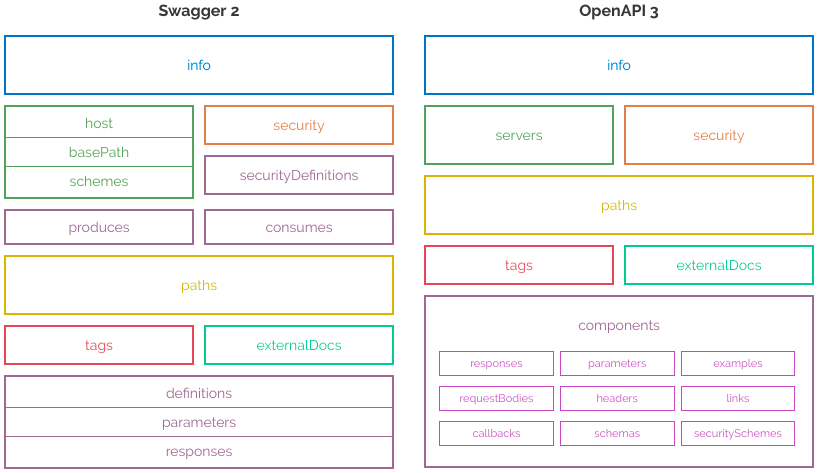
\includegraphics[width=10cm]{openapi2u3.png}
	\caption{Überblick über die Struktur der Open API 2.0 und Open API 3.0 Spezifikationen\cite{openapi2u317}}
	\label{openapi2u317-1}
\end{figure}

\subsection{Neuer Versionsbezeichner}

In 2.0 spec gibt es eine Eigenschaft namens "`swagger"', die die Version der Spezifikation angibt, zum Beispiel:\\

\begin{LaTeXCode}[caption={Version von Swagger},captionpos=b, label=LaTeXCode:swagger2.0-1][numbers=none]
"swagger": "2.0"\\
\end{LaTeXCode}

Die Versionseigenschaft, die von 2.0 als Swagger bezeichnet wurde, wird in Version 3.0 durch eine Versionskennung von Open API ersetzt.\\

\begin{LaTeXCode}[caption={Version von Open API},captionpos=b, label=LaTeXCode:openapi3.0-1][numbers=none]
"openapi": "3.0.0"\\
\end{LaTeXCode}

\subsection{Komponentenobjekte}

OpenAPI 2.0 war im Verhalten von Eigenschaften auf Stammebene etwas inkonsistent und waren nicht so gut definiert. Beispielsweise enthielten einige Eigenschaften Metadaten, die global auf die API angewendet wurden und andere Eigenschaften wurden als Container für wiederverwendbare Fragmente von Metadaten verwendet, auf die an anderer Stelle verwiesen wird. Um dies zu verdeutlichen und die Anzahl der Eigenschaften auf Stammebene zu minimieren, wird eine neue Komponenteneigenschaft eingeführt. Diese Komponenteneigenschaft enthält nur wiederverwendbare Metadaten, auf die an anderer Stelle im Dokument verwiesen wird.\\

Die Liste der OpenAPI 3-Komponenten:

\begin{itemize}
	\item \texttt{responses}
	\item \texttt{parameters}
	\item \texttt{examples}
	\item \texttt{requestBodies}
	\item \texttt{headers}
	\item \texttt{links}
	\item \texttt{callbacks}
	\item \texttt{schemas}
	\item \texttt{securitySchemes}
\end{itemize}

\begin{LaTeXCode}[caption={Komponenten: securitySchemes - Beispiel},captionpos=b, label=LaTeXCode:openapi3.0-1][numbers=none]
"components": {
	"securitySchemes": {
		"api_key": {
			"type": "apiKey",
			"name": "api_key",
			"in": "header"
		},
		"example_auth": {
			"type": "oauth2",
			"flows": {
				"implicit": {
					"authorizationUrl": "http://example.org/api/oauth/dialog",
					"scopes": {
						"write:example": "modify examples in your account",
						"read:example": "read your examples"
					}
				}
			}
		}
	}
}
\end{LaTeXCode}















































